\chapter{Traitement du son}  

Le traitement du son a pour objectif d'améliorer la qualité de signaux au format audio, de les compresser ou encore d'en extraire une information. On distingue généralement les signaux analogiques représentés par des flux continus de données des signaux digitaux représentés par une séquence de symboles binaires.

\section*{Synoptique}

{\footnotesize
\begin{itemize}
\item Logiciel\footnote{Le logiciel Audacity est librement téléchargeable : \url{http://www.audacityteam.org/}} : \emph{Audacity 2.0} 
\item Prérequis : aucun
\item Matières concernées : anglais.
\item Compétences : 
        \begin{itemize}
        \item passer une piste stéréo en mono ;
        \item ajouter une piste ;
        \item copier et coller une partie de piste ;
        \item déplacer une partie de piste (glissement temporel)
        \item rendre silencieuse une partie d'une piste ;
        \item supprimer et raccorder ;
        \item réaliser un fondu en ouverture ou en fermeture ;
        \item exporter un projet au format MP3 ou WAV.
        \end{itemize}
\item Cette fiche est à réaliser :
        \begin{itemize}
	\item avant la fin du semestre de cours en musique (séance 1).
        \item avant les vacances de février en anglais (séance 2) ; 
        \end{itemize}
\end{itemize}
}% fin du footnotesize

\vspace{12pt}
%\section*{Les années précédentes, vous avez appris...}

Les compétences listées ci-dessous ont été vues en classes de 6\up{e} et de 5\up{e}. Vous en aurez à nouveau besoin pour les activités de cette année. Si nécessaire, reportez-vous aux \emph{Fiches MITIC} des années précédentes pour revoir comment :  

\begin{itemize}
\item passer une piste stéréo en mono (5\up{e}) ;
\item ajouter une piste (5\up{e}) ;
\item copier et coller une partie de piste (5\up{e}) ;
\item déplacer une partie de piste (glissement temporel) (5\up{e}) ; 
\item rendre silencieuse une partie d'une piste (5\up{e}) ;
\item supprimer et raccorder (5\up{e}) ;
\item réaliser un fondu en ouverture ou en fermeture (5\up{e}) ;
\item exporter un projet au format MP3 ou WAV (5\up{e}).
\end{itemize}




\section{L'interface graphique d'Audacity (rappel)}\index{Audacity!Interface graphique}\index{Interface graphique (Audacity)}


\begin{itemize}
\item \textbf{La barre de menu principale}\index{Audacity!Barre de menu principale}\index{Barre de menu principale (Audacity)}\label{Son1BarreMenu}

\begin{minipage}[c]{.48\textwidth}
\centering%
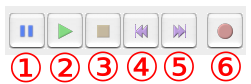
\includegraphics[angle=0,width=.5\textwidth]{./images/son02/barre_1nb}
\end{minipage}\hfill%
\begin{minipage}[c]{.48\textwidth}
\begin{tabular}{lll}
\circled{1} Pause  & & \circled{4} Saut au début \\
\circled{2} Lecture & &\circled{5} Saut à la fin  \\
\circled{3} Stop  & &\circled{6} Enregistrement\\
\end{tabular}
\end{minipage}

\vspace{12pt}\item \textbf{La palette d'outils à disposition}\index{Audacity!Palette d'outils}\index{Palette d'outils (Audacity)}\label{Son1Outils}

\begin{minipage}[c]{.17\textwidth}
\centering%
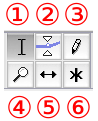
\includegraphics[angle=0,width=.7\textwidth]{./images/son02/barre_2nb}
\end{minipage}\hfill%
\begin{minipage}[c]{.78\textwidth}
\begin{tabular}{p{6cm}lp{6cm}}
\circled{1} Outil de sélection : permet de sélectionner une région && \circled{4} Outil de zoom \\
\circled{2} Outil de niveau (enveloppe) : permet de changer le volume localement && \circled{5} Outil de glissement temporel : permet de déplacer dans le temps l'enregistrement \\
\circled{3} Outil de dessin d'onde : permet de modifier la forme de l'onde && \circled{6} Mode multi-outils \\
\end{tabular}
\end{minipage}

\vspace{12pt}\item \textbf{Réglage des volumes d'entrée/sortie}\index{Audacity!Réglage des volumes}\index{Réglage des volumes (Audacity)}

Les vu-mètres de sortie 
\includegraphics[angle=0,width=.6cm]{./images/son02/hp} et d'entrée 
\includegraphics[angle=0,width=.6cm]{./images/son02/micro} (figure à gauche ci-dessous) permettent de visualiser le volume de sortie ou d'enregistrement. Si ceux-ci ne sont pas satisfaisants (trop faibles ou saturation), alors il est possible de les ajuster grâce aux deux glissières voisines (figure à droite ci-dessous).

\deuximagesici{./images/son02/barre_3}{.8\textwidth}{./images/son02/barre_4}{.8\textwidth}    


La glissière accompagnant la flèche verte (
\includegraphics[angle=0,width=.4cm]{./images/son02/fleche_verte}) permet de modifier la vitesse de lecture.

\end{itemize}



\subsection{Exporter un projet au format MP3 ou WAV (rappel)}\index{Audacity!Exporter en MP3 ou WAV}\index{MP3 export (Audacity)}\index{WAV export (Audacity)} 

Pour exporter un projet au format MP3 (format compressé avec pertes) ou WAV (format non compressé), il faut se rendre dans le menu \texttt{Fichier} puis choisir \texttt{Exporter...}

\vspace{6pt}

Dans la boîte de dialogue qui s'ouvre alors, choisir le nom du fichier (\circled{1} sur la figure ci-dessous), l'emplacement où le fichier doit être enregistré \circled{2} (ici le \texttt{Bureau}), le format du fichier \circled{3} (ici le projet sera exporté au format MP3, mais il est également possible de choisir le format WAV), puis cliquer sur le bouton \texttt{OK} \circled{4}.       

\uneimageici{./images/son02/audacityExporter}{.8\textwidth}

Pour les boîtes de dialogues suivantes, conserver les options par défaut et cliquer sur le bouton \texttt{OK} pour réaliser l'export. 



%
%
%  S  É  A  N  C  E     I
%
%

\pagebreak

\section{Séance 1 : Musique}\label{ficheSon4e1}

\boiteEnonceLarge{%
Le but est de supprimer la voix dans une chanson.
} % fin énoncé

\vfill

\cadre{Pensez à sauver régulièrement votre travail en appuyant sur \texttt{Cmd + S} ou à partir du menu \texttt{Fichier} en choisissant \texttt{Enregistrer}.

\uneimageici{./images/generales/clavierCmdS}{.5\textwidth}
}




%
%
%  S  É  A  N  C  E     II
%
%


\pagebreak

\section{Séance 2 : Anglais}\label{ficheSon4e2}

\boiteEnonceLarge{%
Énoncé de la séance 2
}% fin énoncé

\vfill

\cadre{Pensez à sauver régulièrement votre travail en appuyant sur \texttt{Cmd + S} ou à partir du menu \texttt{Fichier} en choisissant \texttt{Enregistrer}.

\uneimageici{./images/generales/clavierCmdS}{.5\textwidth}
}


%
%
%  S  É  A  N  C  E     III
%
%






